\section{ATMS Response Data}
%===========================

\subsection{Specified and measured responses}
%--------------------------------------------
The NPP ATMS specified central frequencies, sideband offsets and channel bandwidths, taken from table 9 of the CrIS EDR ATBD\cite{CrIS_EDR_ATBD}, are shown in table \ref{tab:atms_fo_sb_and_df}. Also shown are measured bandwidths taken from table 12-1 of the ATMS PFM Calibration Data Book\cite{ATMS_PFM_CalLog}. No measurements of the central frequencies are readily available \footnote{These values may be available in other ATMS reports, particularly: RE-13680 K/Ka Band Receiver Shelf Verification Report, RE-13658 W Band Receiver Shelf Verification Report, RE-13741 V Band Receiver Shelf Verification Report, and RE-13802 G Band Receiver Shelf Verification Report.}. These frequency parameters are used to construct the so-called ``boxcar'' spectral response functions. 

Note that the bandpass information presented in Table VII of the ATMS Receiver Specification\cite{ATMS_Receiver_Spec} is not used here because the sideband frequency offset for channel 17 ($\pm$1500MHz) is incorrect. Because no supplemental passband information from the referenced Table VII\cite{ATMS_Receiver_Spec} was used, channels 10 and 17 appear as single passband channels in table \ref{tab:atms_fo_sb_and_df}.

\begin{table}[htp]
  \centering
  \begin{tabular}{c c c c c c}
    \hline
                     & \textbf{Central}         & \textbf{Sideband 1}   & \textbf{Sideband 2}   & \textbf{Specified}       & \textbf{Measured} \\
                     & \textbf{Frequency}\up{a} & \textbf{Offset}\up{a} & \textbf{Offset}\up{a} & \textbf{Bandwidth}\up{a} & \textbf{Bandwidth}\up{b} \\
    \textbf{Channel} & \bfrequency{0}           & \bsideband{1}         & \bsideband{2}         & \bdeltaf                 & \bdeltaf      \\
                     & (GHz)                    & (GHz)                 & (GHz)                 & (GHz)                    & (GHz)         \\
    \hline\hline
            1        &  23.800000  & -      & -      & 0.27   & 0.258         \\
            2        &  31.400000  & -      & -      & 0.18   & 0.172         \\
            3        &  50.300000  & -      & -      & 0.18   & 0.173         \\
            4        &  51.760000  & -      & -      & 0.40   & 0.381         \\
            5        &  52.800000  & -      & -      & 0.40   & 0.366         \\
            6        &  53.596000  & 0.115  & -      & 0.17   & 0.1587,0.1648\up{c} \\
            7        &  54.400000  & -      & -      & 0.40   & 0.387         \\
            8        &  54.940000  & -      & -      & 0.40   & 0.387         \\
            9        &  55.500000  & -      & -      & 0.33   & 0.317         \\
           10        &  57.290344  & -      & -      & 0.33   & 0.151         \\
           11        &  57.290344  & 0.217  & -      & 0.078  & 0.0763        \\
           12        &  57.290344  & 0.3222 & 0.048  & 0.036  & 0.0351        \\
           13        &  57.290344  & 0.3222 & 0.022  & 0.016  & 0.01547       \\
           14        &  57.290344  & 0.3222 & 0.010  & 0.008  & 0.0078,0.0079\up{c} \\
           15        &  57.290344  & 0.3222 & 0.0045 & 0.003  & 0.0029        \\
           16        &  88.200000  & -      & -      & 2.0    & 1.9282        \\
           17        & 165.500000  & -      & -      & 3.0    & 1.1251        \\
           18        & 183.310000  & 7.0    & -      & 2.0    & 1.9302        \\
           19        & 183.310000  & 4.5    & -      & 2.0    & 1.9519        \\
           20        & 183.310000  & 3.0    & -      & 1.0    & 0.9799        \\
           21        & 183.310000  & 1.8    & -      & 1.0    & 0.9823        \\
           22        & 183.310000  & 1.0    & -      & 0.5    & 0.4940        \\
    \hline
  \end{tabular}
  \caption{Central, sideband offset, and bandwidth frequencies for ATMS. \superscript{a}Data from table 9 of ref.\cite{CrIS_EDR_ATBD}. \superscript{b}Data from table 12-1 of ref.\cite{ATMS_PFM_CalLog}. \superscript{c}Different lower and upper sideband widths reported. }
  \label{tab:atms_fo_sb_and_df}
\end{table}


\subsection{Measured frequency filter responses}
%-----------------------------------------------
In addition to the usual frequency parameters, the ATMS PFM Calibration Data Book\cite{ATMS_PFM_CalLog} contains tables (12-2a to 12-2d) of the digitised filter responses (hereafter referred to as spectral response functions, or SRFs). It should be noted that these ``Table 12'' SRFs are for the frequency filter response only and are not necessarily indicative of the system response. As such, none of the Table 12 SRFs were used in the analyses presented in this Office Note and are only mentioned here for the record. A selection of four channels from the Table 12 ATMS SRF data, compared to the boxcar response, is shown in figure \ref{fig:table12.srf_selection}. All of the channel Table 12 SRFs are shown in appendix \ref{app:srf.table12}.

\begin{figure}[htp]
  \centering
  \begin{tabular}{c c}
    \textsf{\textbf{(a)} Channel 6} &
    \textsf{\textbf{(b)} Channel 10} \\
    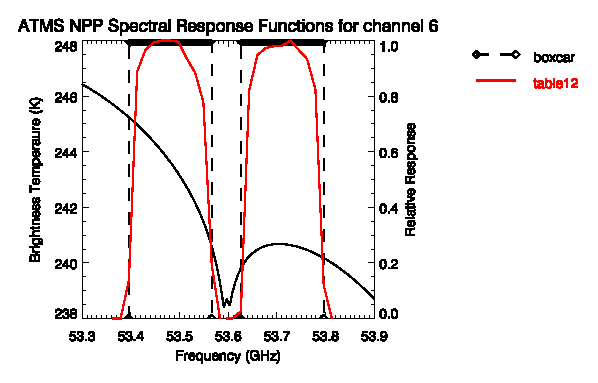
\includegraphics[bb=70 400 300 559,clip,scale=1.0]{graphics/srf/table12/atms_npp.ch6.osrf.eps} &
    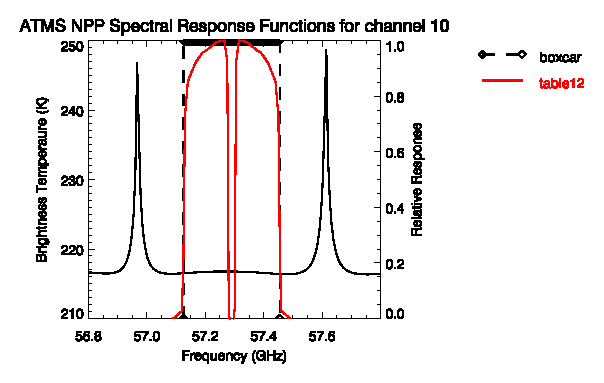
\includegraphics[bb=70 400 300 559,clip,scale=1.0]{graphics/srf/table12/atms_npp.ch10.osrf.eps} \\\\

    \textsf{\textbf{(c)} Channel 11} &
    \textsf{\textbf{(d)} Channel 19} \\
    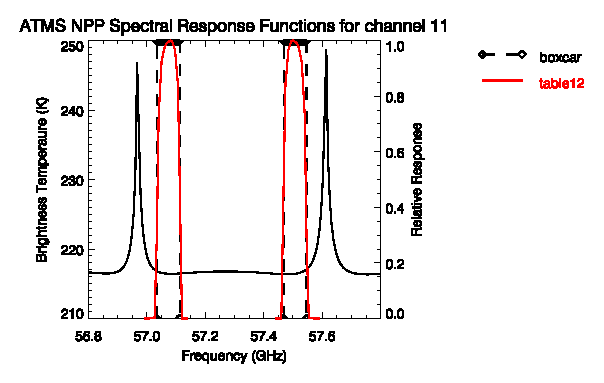
\includegraphics[bb=70 400 300 559,clip,scale=1.0]{graphics/srf/table12/atms_npp.ch11.osrf.eps} &
    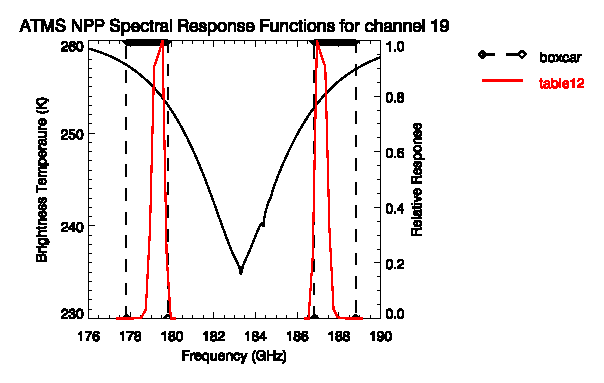
\includegraphics[bb=70 400 300 559,clip,scale=1.0]{graphics/srf/table12/atms_npp.ch19.osrf.eps}
  \end{tabular}
  \caption{Selection of NPP ATMS Table 12 SRF data from the ATMS PFM Calibration Data Book\cite{ATMS_PFM_CalLog} with the corresponding boxcar response based on table \ref{tab:atms_fo_sb_and_df} data. A representative brightness temperature spectrum is also shown. See Appendix \ref{app:srf.table12} for the Table 12 SRFs for all channels.}
  \label{fig:table12.srf_selection}
\end{figure}


\subsection{Additional Digitised Responses}
%------------------------------------------
After the first NPOESS SOAT meeting\footnote{Sounding Operational Algorithm Team (SOAT) Meeting, CrIS/ATMS Cal/Val Team, Integrated Program Office, Silver Spring, Maryland, USA, 20-21 May 2009} where the NPP ATMS Table 12 SRF data was discussed, two of us (DeAmici, NGAS; Chidester, SDL) began digitizing the graphical SRFs displayed in the ATMS PFM Calibration Data Book\cite{ATMS_PFM_CalLog}. Different SRF datasets were digitized based upon the baseplate temperature (-10\textdegree{}C, 20\textdegree{}C, and 50\textdegree{}C) and the bias voltages supplied to the amplifiers, oscillators, and pre-amplifiers (low, nominal, and high). Additionally, separate digitizations for some temperature/voltage combinations were performed for both the low and high spectral resolution measurements displayed in \cite{ATMS_PFM_CalLog}.

The difference between the low and high resolution SRFs in \cite{ATMS_PFM_CalLog} is that, for the former, a greater range of response data was plotted (typically extending below -40dB insertion loss) requiring a larger bandwidth and including the ``wings'' of the SRFs and, for the latter, the plots typically only displayed responses \emph{just} beyond the frequencies marking the -3dB insertion loss point (which corresponds roughly to the half-maximum of the SRF). The available digitized SRF datasets are shown in table \ref{tab:RESlow_datasets} for low spectral resolution, and table \ref{tab:RESlow_datasets} for high spectral resolution.

\begin{table}[htp]
  \centering
  \begin{tabular}{c c c c }
    \hline
          & \textbf{V\subscript{low}} & \textbf{V\subscript{nom}} & \textbf{V\subscript{high}} \\
    \hline\hline
    \textbf{-10\textdegree{}C} &  x  & SDL &  x  \\
    \textbf{ 20\textdegree{}C} & SDL & SDL & SDL \\
    \textbf{ 50\textdegree{}C} &  x  & SDL &  x  \\
     \hline
  \end{tabular}
  \caption{Low spectral resolution digitized SRF datasets.}
  \label{tab:RESlow_datasets}
\end{table}

\begin{table}[htp]
  \centering
  \begin{tabular}{c c c c }
    \hline
          & \textbf{V\subscript{low}} & \textbf{V\subscript{nom}} & \textbf{V\subscript{high}} \\
    \hline\hline
    \textbf{-10\textdegree{}C} &  x  & SDL  &  x  \\
    \textbf{ 20\textdegree{}C} &  x  & NGAS & SDL \\
    \textbf{ 50\textdegree{}C} &  x  &  x   &  x  \\
     \hline
  \end{tabular}
  \caption{High spectral resolution digitized SRF datasets.}
  \label{tab:REShi_datasets}
\end{table}


\subsection{Conversion of insertion loss to relative response}
%-------------------------------------------------------------
Convolution of line-by-line (LBL) radiance calculations with the SRFs to produce the channel radiance, $\overline{R}$, is done using
\begin{equation}
  \overline{R} = \frac{\displaystyle\int_{\nu_1}^{\nu_2}R(\nu)\phi(\nu)d\nu}{\displaystyle\int_{\nu_1}^{\nu_2}\phi(\nu)d\nu}
  \label{eqn:radiance_convolution}
\end{equation}
where $R(\nu)$ is the LBL radiance at frequency $\nu$, $\phi(\nu)$ is the SRF relative response, and $\nu_1,\nu_2$ are the frequency bounds of the SRF in units of inverse centimetres (cm\superscript{-1}).

The SRF magnitudes in the ATMS PFM Calibration Data Book\cite{ATMS_PFM_CalLog} are described in terms of insertion loss in units of decibels, $L_{dB}$. The relationship between insertion loss and relative response is taken to be,
\begin{equation}
  L_{dB}(\nu) = 10\log_{10}\left(\displaystyle\frac{\phi(\nu)}{\phi_0}\right)
  \label{eqn:response_to_db}
\end{equation}
where the ``reference'' relative response, $\phi_0$, is set to 1.0. Coupling this with a rearrangment of equation \ref{eqn:response_to_db} gives,
\begin{equation}
  \phi(\nu) = 10^{0.1L_{dB}(\nu)}
  \label{eqn:db_to_response}
\end{equation}


\subsection{Comparison Datasets}
%-------------------------------
The comparison between the different SRF sets shown here will be split into three groups based on differences in temperature, voltage, and spectral resolution respectively, like so:

\begin{description}
  \item[Temperature comparison (Tset):] Low, nominal, and high base plate temperatures (-10\textdegree{}C, 20\textdegree{}C, 50\textdegree{}C) for nominal bias voltage (V\subscript{nom}) and low spectral resolution (R\subscript{low}).
  \item[Voltage comparison (Vset):] Low, nominal, and high bias voltages (V\subscript{low}, V\subscript{nom}, V\subscript{high}) for nominal baseplate temperature (20\textdegree{}C) and low spectral resolution (R\subscript{low.}).
  \item[Resolution comparison (Rset):] Low and ``effective'' high spectral resolution (R\subscript{low}, R\subscript{high}) for nominal baseplate temperature (20\textdegree{}C) and high bias voltage (V\subscript{high}). The high resolution  is listed as effective since the actual comparisons were done between the original low spectral resolution dataset, and a dataset derived from the low resolution data but truncated at -10dB (equivalent to a relative response of 0.1). Doing this removed the effect of digitization errors from the examination of the impact of the inclusion of the SRF wings.
\end{description}

As with the Table 12 responses shown in figure \ref{fig:table12.srf_selection}, the same selection of channels for the different SRF datasets described above are shown in figures \ref{fig:Tset.srf_selection},  \ref{fig:Vset.srf_selection}, and \ref{fig:Rset.srf_selection} for the Tset, Vset, and Rset comparisons respectively. It is clear from these selected channels that the various actual channel responses are relatively similar, but the all differ significantly from the ``boxcar'' response - in particular those seen for channel 19 (indeed, all the 183GHz channel SRFs exhibit large differences from a boxcar reposnse).

\begin{figure}[htp]
  \centering
  \begin{tabular}{c c}
    \textsf{\textbf{(a)} Channel 6} &
    \textsf{\textbf{(b)} Channel 10} \\
    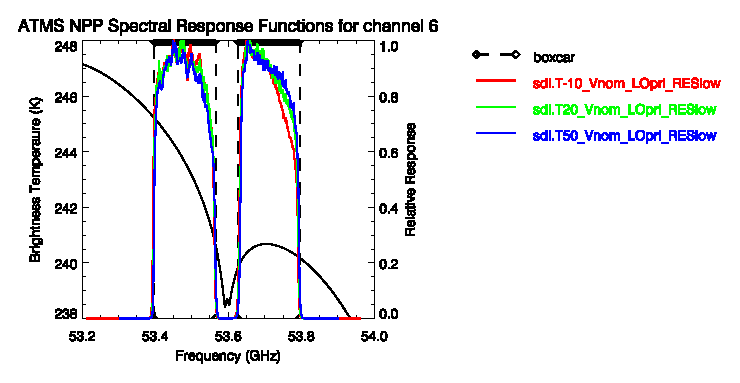
\includegraphics[bb=70 400 300 559,clip,scale=1.0]{graphics/srf/Tset/atms_npp.ch6.osrf.eps} &
    \includegraphics[bb=70 400 300 559,clip,scale=1.0]{graphics/srf/Tset/atms_npp.ch10.osrf.eps} \\\\

    \textsf{\textbf{(c)} Channel 11} &
    \textsf{\textbf{(d)} Channel 19} \\
    \includegraphics[bb=70 400 300 559,clip,scale=1.0]{graphics/srf/Tset/atms_npp.ch11.osrf.eps} &
    \includegraphics[bb=70 400 300 559,clip,scale=1.0]{graphics/srf/Tset/atms_npp.ch19.osrf.eps}
  \end{tabular} \\
  % the hand-crafted legend
  \setlength{\unitlength}{1cm}
  \begin{picture}(8.0,1.0)
    \thicklines
    \color{red}
    \put(0.0,0.5){\line(1,0){1}}
    \put(1.2,0.35){\sffamily -10\textdegree{}C}
    \color{green}
    \put(3.0,0.5){\line(1,0){1}}
    \put(4.2,0.35){\sffamily 20\textdegree{}C}
    \color{blue}
    \put(6.0,0.5){\line(1,0){1}}
    \put(7.2,0.35){\sffamily 50\textdegree{}C}
  \end{picture}
  \caption{Selection of NPP ATMS SRF data from the ATMS PFM Calibration Data Book\cite{ATMS_PFM_CalLog} for the baseplate temperature comparison dataset (Tset), along with the corresponding boxcar response based on table \ref{tab:atms_fo_sb_and_df} data. A representative brightness temperature spectrum is also shown. See Appendix \ref{app:Tset} for the Tset SRFs for all channels.}
  \label{fig:Tset.srf_selection}
\end{figure}

\begin{figure}[htp]
  \centering
  \begin{tabular}{c c}
    \textsf{\textbf{(a)} Channel 6} &
    \textsf{\textbf{(b)} Channel 10} \\
    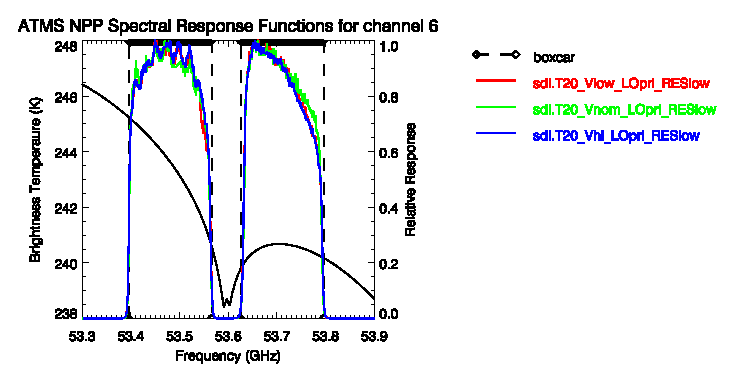
\includegraphics[bb=70 400 300 559,clip,scale=1.0]{graphics/srf/Vset/atms_npp.ch6.osrf.eps} &
    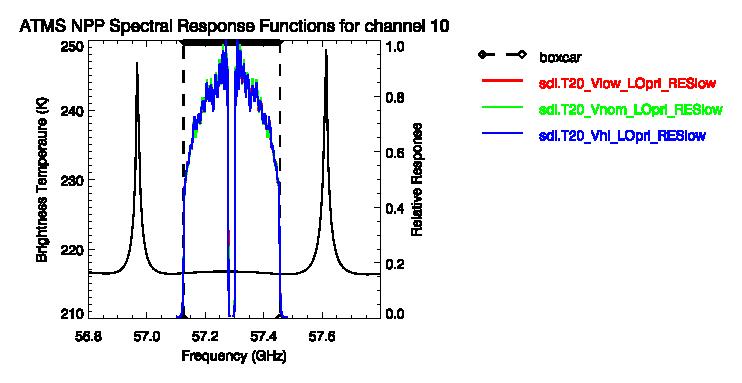
\includegraphics[bb=70 400 300 559,clip,scale=1.0]{graphics/srf/Vset/atms_npp.ch10.osrf.eps} \\\\

    \textsf{\textbf{(c)} Channel 11} &
    \textsf{\textbf{(d)} Channel 19} \\
    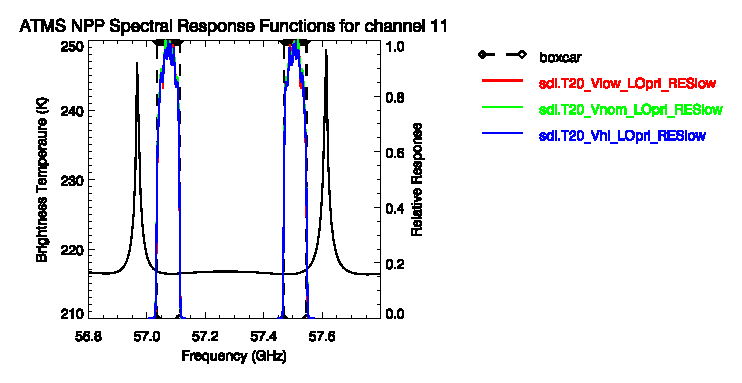
\includegraphics[bb=70 400 300 559,clip,scale=1.0]{graphics/srf/Vset/atms_npp.ch11.osrf.eps} &
    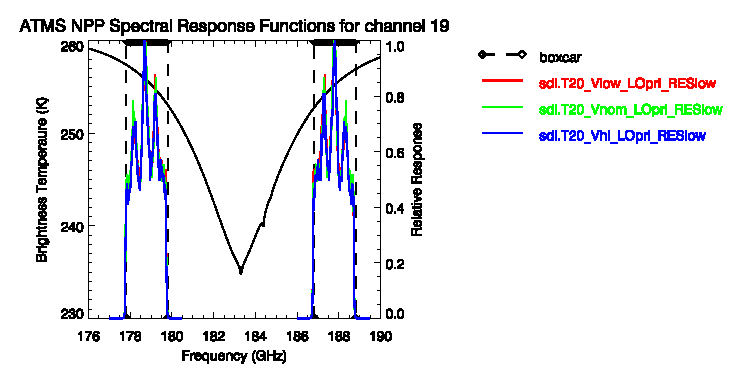
\includegraphics[bb=70 400 300 559,clip,scale=1.0]{graphics/srf/Vset/atms_npp.ch19.osrf.eps}
  \end{tabular} \\
  % the hand-crafted legend
  \setlength{\unitlength}{1cm}
  \begin{picture}(8.0,1.0)
    \thicklines
    \color{red}
    \put(0.0,0.5){\line(1,0){1}}
    \put(1.2,0.35){\sffamily Vlow}
    \color{green}
    \put(3.0,0.5){\line(1,0){1}}
    \put(4.2,0.35){\sffamily Vnom}
    \color{blue}
    \put(6.0,0.5){\line(1,0){1}}
    \put(7.2,0.35){\sffamily Vhigh}
  \end{picture}
  \caption{Selection of NPP ATMS SRF data from the ATMS PFM Calibration Data Book\cite{ATMS_PFM_CalLog} for the bias voltage comparison dataset (Vset), along with the corresponding boxcar response based on table \ref{tab:atms_fo_sb_and_df} data. A representative brightness temperature spectrum is also shown. See Appendix \ref{app:Vset} for the Vset SRFs for all channels.}
  \label{fig:Vset.srf_selection}
\end{figure}

\begin{figure}[htp]
  \centering
  \begin{tabular}{c c}
    \textsf{\textbf{(a)} Channel 6} &
    \textsf{\textbf{(b)} Channel 10} \\
    \includegraphics[bb=70 400 300 559,clip,scale=1.0]{graphics/srf/Rset/atms_npp.ch6.osrf.eps} &
    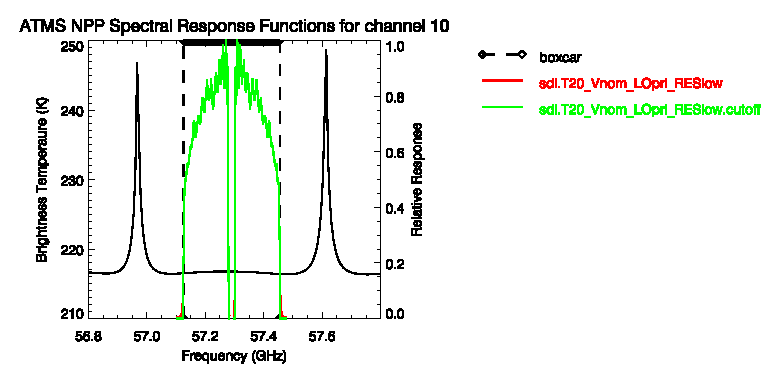
\includegraphics[bb=70 400 300 559,clip,scale=1.0]{graphics/srf/Rset/atms_npp.ch10.osrf.eps} \\\\

    \textsf{\textbf{(c)} Channel 11} &
    \textsf{\textbf{(d)} Channel 19} \\
    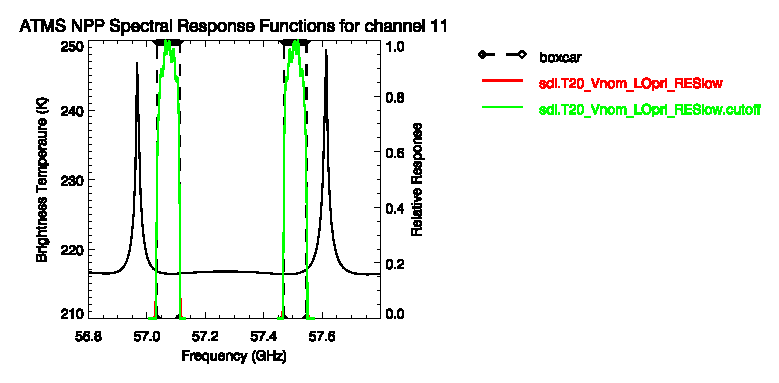
\includegraphics[bb=70 400 300 559,clip,scale=1.0]{graphics/srf/Rset/atms_npp.ch11.osrf.eps} &
    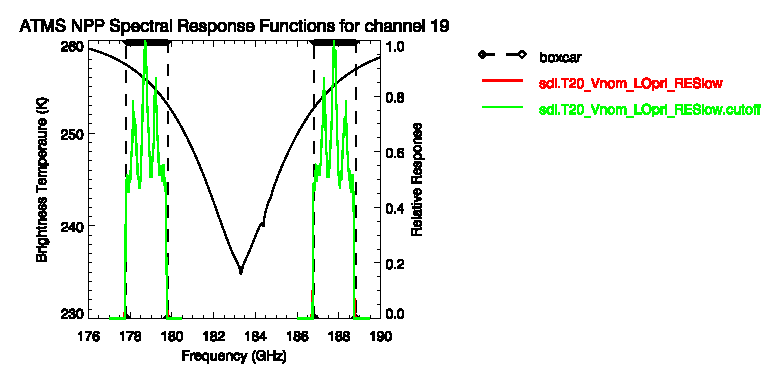
\includegraphics[bb=70 400 300 559,clip,scale=1.0]{graphics/srf/Rset/atms_npp.ch19.osrf.eps}
  \end{tabular} \\
  % the hand-crafted legend
  \setlength{\unitlength}{1cm}
  \begin{picture}(9.0,1.0)
    \thicklines
    \color{red}
    \put(0.0,0.5){\line(1,0){1}}
    \put(1.2,0.35){\sffamily SRF wings included}
    \color{green}
    \put(5.0,0.5){\line(1,0){1}}
    \put(6.2,0.35){\sffamily SRF cutoff at -10dB}
  \end{picture}
  \caption{Selection of NPP ATMS SRF data from the ATMS PFM Calibration Data Book\cite{ATMS_PFM_CalLog} for the 20\textdegree{}C, Vnominal spectral resolution dataset (Rset), along with the corresponding boxcar response based on table \ref{tab:atms_fo_sb_and_df} data. A representative brightness temperature spectrum is also shown. See Appendix \ref{app:Rset} for the Rset3 SRF for all channels.}
  \label{fig:Rset.srf_selection}
\end{figure}
